\clearpage
\section{Liturgical Books and Stands}
In the postconciliar Roman Rite, the single 1962 altar Missal was divided into distinct ritual volumes reflecting the structure of Mass: the Roman Missal for presidential prayers and the Eucharistic Prayer, the Lectionary for the three-year Sunday and two-year weekday Scripture cycles, the ornate Book of the Gospels carried in solemn procession, and in the United States the lighter Book of the Chair for presidential prayers away from the altar.

\PCDPlateHeader{Plate V --- Liturgical Books and Stands}{Relative proportions shown}
\ifdefined\TriptychPrintEdition
\begin{center}
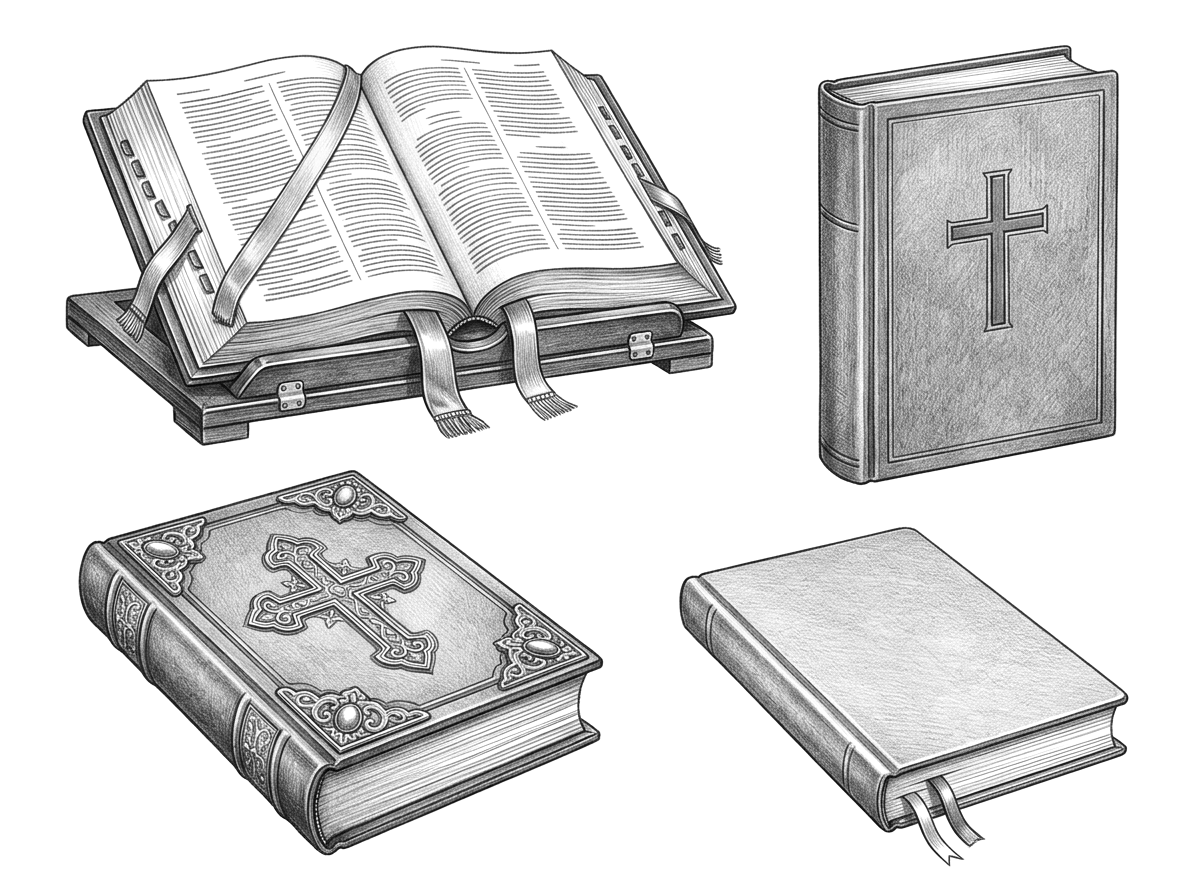
\includegraphics[width=0.92\linewidth,height=3.55in,keepaspectratio]{liturgy/roman-rite/postconciliar/2008-latin-2011-us-english/reference/roman-sanctuary-dictionary/shared/artwork/graphite/pc-art-05-liturgical-books.png}
\end{center}
\PCDPositionKey{Top left: thick Roman Missal open with side tabs and ribbon markers on a low angled Missal Stand; top right: tall closed Lectionary for Mass; bottom left: ornate bound Book of the Gospels (Evangeliary) with metal corner bosses and embossed cross; bottom right: slimmer Book of the Chair (Excerpts from the Roman Missal).}
\else
\textbf{Visual Plate Summary (Plate V --- Liturgical Books and Stands, Relative proportions shown):} Four-book monochrome graphite comparison showing relative scale and binding dignity: top left, a thick altar Roman Missal open flat with ribbon markers and edge tabs on a low angled wooden stand; top right, a tall closed hardcover Lectionary marked with a plain cover cross; bottom left, a heavily ornamented Book of the Gospels with sculpted metal corner bosses and central embossed cross; bottom right, a slimmer handheld Book of the Chair with two ribbon markers.

\textbf{Reading order and object placement:} Top left: thick Roman Missal open with side tabs and ribbon markers on a low angled Missal Stand; top right: tall closed Lectionary for Mass; bottom left: ornate bound Book of the Gospels (Evangeliary) with metal corner bosses and embossed cross; bottom right: slimmer Book of the Chair (Excerpts from the Roman Missal).
\fi

\label{pc-obj-roman-missal}
\PCDEntryHead{Roman Missal}{Missale Romanum}{required}{N20}
\PCDField{Also called}{Altar Missal; Sacramentary (1974--2011 U.S. usage); \textit{Missale}}
The principal liturgical book of the Roman Rite containing the Order of Mass, Eucharistic Prayers, Prefaces, presidential prayers, antiphons, and rubrics proclaimed by the priest celebrant. At top left of Plate V, the heavy altar Missal lies open flat in two-column pages on a low wooden stand, fitted with durable side tabs along both fore-edges and multiple fringed silk ribbon markers. Ordinarily bound in red leather or cloth with sturdy sewing, it is thicker and heavier than the other sanctuary volumes shown in relative proportion on Plate V.

\PCDField{Plate position and status}{Top left, open with edge tabs and ribbons on a low stand (Plate V) (Universal Roman law)}
\PCDField{Placement and liturgical use}{Prepared beside the presidential chair before Mass (GIRM 118a, unless the Book of the Chair is used for chair prayers) and placed on the altar at the Preparation of the Gifts so the priest prays the Prayer over the Offerings, Preface, Eucharistic Prayer, and Communion rites directly from it (GIRM 139, 306). After the purification of vessels, it may return to the presidential chair for the Prayer after Communion and Solemn Blessing (GIRM 165--167, 306).}
\PCDField{United States norm}{In the Dioceses of the United States of America, the approved vernacular edition is The Roman Missal, Third Edition (USCCB, effective 27 November 2011), translating the 2002/2008 Latin third typical edition in its entirety (GIRM 389) and incorporating confirmed United States adaptations and the 2021 emendations.}
\PCDField{Ministers and server boundary}{Ordinary ministers: Bishop, Priest. Server carries and presents to priest or deacon: Servers check ribbon markers before Mass as directed, hold the open Roman Missal steady at chest or reading height for the priest at the presidential chair when no stand or Book of the Chair is used, place it cleanly on the altar at the Preparation of the Gifts, and remove it after purification when instructed.}
\PCDSafety{Support the heavy altar Missal evenly with both hands or braced cleanly against your upper chest---never by one cover---so the binding does not tear or slip. Never set loose announcements, bulletins, or unapproved sheets atop the Missal or on the altar mensa (GIRM 306).}
\PCDField{Distinguish from}{Book of the Chair, Lectionary for Mass, Book of the Gospels}
\PCDField{Symbolism}{The General Instruction of the Roman Missal teaches that liturgical books serve as signs and symbols of heavenly realities, requiring that the Roman Missal be crafted with genuine worth, dignity, and beauty to honor the Eucharistic prayer of the Church. (GIRM 349)}
\PCDField{1962 Roman Missal counterpart}{\PCDTag{materially changed} The 1962 Missale Romanum was a plenary altar book holding all presidential orations, chants, Epistles, and Gospels, remaining on the altar throughout Mass and carried between the Epistle and Gospel corners (RG 527; RS VI.5, XI.1). In the postconciliar Roman Rite, the Scripture readings are separated into the Lectionary and Book of the Gospels, while the Missal serves at the presidential chair and rests on the altar only from the Preparation of the Gifts through purification (GIRM 118a, 139, 306).}
\PCDEntryRule

\label{pc-obj-lectionary}
\PCDEntryHead{Lectionary for Mass}{Lectionarium}{required}{N21}
\PCDField{Also called}{Lectionary; \textit{Ordo lectionum Missae}}
The official ritual book of Sacred Scripture containing the appointed first and second readings, Responsorial Psalms, Gospel Acclamations, and Gospels organized across the three-year Sunday cycle (Years A, B, and C) and two-year weekday cycle (Years I and II). At top right of Plate V, the closed Lectionary stands upright as a tall, dignified hardcover ritual volume with a plain rectangular border and simple central cross stamped on the cover---stately in proportion, yet visibly less ornate than the metal-bossed Book of the Gospels directly below it.

\PCDField{Plate position and status}{Top right, tall closed volume with cover cross (Plate V) (Universal Roman law)}
\PCDField{Placement and liturgical use}{Placed open to the day's readings on the stationary ambo before Mass begins (GIRM 118b). Instituted lectors and deputed readers proclaim the first and second readings from it at the ambo, and the deacon or priest proclaims the Gospel from it whenever a separate Book of the Gospels is not employed. Under universal Roman rubrics (GIRM 120d, 194), the Lectionary is never carried in the entrance procession---only the Book of the Gospels receives that ceremonial procession.}
\PCDField{United States norm}{In the Dioceses of the United States of America, Scripture readings at Mass are proclaimed from the approved Lectionary for Mass for Use in the Dioceses of the United States (Confraternity of Christian Doctrine), arranged according to the 1981 editio typica altera of the Ordo lectionum Missae; disposable booklets or parish missalettes never replace the ritual Lectionary on the ambo (GIRM 349; OLM 35--37).}
\PCDField{Ministers and server boundary}{Ordinary ministers: Bishop, Priest, Deacon, Instituted lector. Server prepares or sets in place before or during Mass: Servers may confirm before Mass that the Lectionary lies open to the appointed day's readings on the ambo and may return it to the sacristy after Mass; servers never carry the Lectionary in the entrance procession and never proclaim Scripture from it unless separately deputed as readers.}
\PCDSafety{Never carry the Lectionary in the entrance procession---GIRM 120d and 194 strictly reserve the entrance book procession to the Book of the Gospels. Never replace the ritual Lectionary on the ambo with disposable paper leaflets or pew missalettes (GIRM 349).}
\PCDField{Distinguish from}{Book of the Gospels, Roman Missal}
\PCDField{Symbolism}{The General Instruction of the Roman Missal honors the Lectionary alongside the Book of the Gospels as a sign and symbol of heavenly realities serving the proclamation of God's Word, feeding the faithful at the table of God's Word before the table of Christ's Body. In the words of the psalmist, ``Thy word is a lamp to my feet, and a light to my paths'' (Ps 118:105 [119:105]). (GIRM 28, 349; Ordo lectionum Missae (1981) Praenotanda 35; Ps 118:105 [119:105])}
\PCDField{1962 Roman Missal counterpart}{\PCDTag{materially changed} In the 1962 Roman Missal, the one-year cycle of Epistles and Gospels was printed inside the Missal itself, with an optional separate Epistle book (liber Epistolarum) for the subdeacon at Solemn Mass (RS VI.4). The postconciliar reform established a dedicated multi-volume Lectionary spanning a three-year Sunday cycle (A, B, C) and two-year weekday cycle (I, II), placed open on the ambo for every Mass with a congregation (GIRM 118b; OLM 1981).}
\PCDEntryRule

\label{pc-obj-book-of-the-gospels}
\PCDEntryHead{Book of the Gospels}{Evangeliarium}{provided}{N22}
\PCDField{Also called}{Evangeliary; Gospel Book; \textit{Liber Evangeliorum}}
A dedicated, richly ornamented ritual volume containing solely the liturgical Gospels, accorded supreme ceremonial honor among all sanctuary books through entrance procession, placement on the altar, escorted procession to the ambo with candles and incense, and reverent kissing after proclamation. At bottom left of Plate V, the closed Book of the Gospels stands out immediately from the plainer Lectionary by its heavy embossed cover, sculpted metal corner bosses, raised spine bands, and prominent floriated cross in relief.

\PCDField{Plate position and status}{Bottom left, ornate metal-bossed cover (Plate V) (Universal Roman law)}
\PCDField{Placement and liturgical use}{Strongly commended for cathedrals and parishes (OLM 36). Carried slightly elevated in the entrance procession by the deacon---or, in the deacon's absence, by an instituted or deputed lector---and laid flat on the center of the altar, the sole book permitted upon the mensa from the beginning of Mass until the Gospel (GIRM 120d, 122, 172--173, 194, 306). At the Gospel Acclamation, the deacon (or priest, if no deacon serves) lifts it from the altar and carries it to the ambo accompanied by servers with lighted candles and incense; after three swings of incense (GIRM 277; executed as paired double swings in Roman ceremonial custom, Caeremoniale Episcoporum 92) and proclamation, the minister reverently kisses the book while praying quietly Per evangelica dicta (GIRM 134, 175).}
\PCDField{United States norm}{In the Dioceses of the United States of America, the approved Book of the Gospels contains the Sunday and feast-day Gospels in the Lectionary translation and is customarily bound in embossed metallic or richly ornamented covers honoring the dignity commended by GIRM 349 and OLM 36--37.}
\PCDField{Ministers and server boundary}{Ordinary ministers: Bishop, Priest, Deacon, Instituted lector. Server recognizes only; does not handle: Altar servers never carry the Book of the Gospels in the entrance procession (reserved strictly to the deacon, or to an instituted or deputed lector if no deacon is present) and never lift it from the altar for the Gospel procession; servers escort it with lighted candles and the thurible, flank the ambo during proclamation, and may reverently return the closed volume to the sacristy after Mass.}
\PCDSafety{Never hand the Book of the Gospels to an altar server to carry in the entrance procession---GIRM 120d and 194 reserve that role strictly to the deacon or, in his absence, a lector. During the Gospel procession, candle-bearers hold flames well clear of the ornate cover and open pages.}
\PCDField{Distinguish from}{Lectionary for Mass, Roman Missal}
\PCDField{Symbolism}{First among all liturgical books as a sign and symbol of heavenly realities, the Book of the Gospels receives elevation in procession, placement upon the altar, escort with lights and incense, and a reverent kiss because Christ himself speaks directly to his Church in the Gospel. St. Thomas Aquinas similarly distinguishes the earlier readings as preparatory instruction from the Gospel, by which Christ's own teaching instructs the faithful perfectly. (GIRM 62, 134, 175, 349; St. Thomas Aquinas, Summa Theologiae III, q. 83, a. 4, corpus)}
\PCDField{1962 Roman Missal counterpart}{\PCDTag{changed use} In the 1962 Roman Missal, a separate Gospel book (liber Evangeliorum) belonged to Solemn Mass, where it was placed on the altar only before the Gospel, carried by the deacon in the Gospel procession, held by the subdeacon between lighted candles, incensed, and brought to the celebrant to kiss (RS VI.5). Postconciliar rubrics integrate the Book of the Gospels into ordinary Sunday and festive celebrations, carrying it slightly elevated in the entrance procession and resting it on the altar from the start of Mass until the Gospel procession (GIRM 120d, 122, 133--134, 306).}
\PCDEntryRule

\label{pc-obj-book-of-the-chair}
\PCDEntryHead{Book of the Chair}{Excerpts from the Roman Missal (no Latin typical edition)}{territorial adaptation}{N23}
\PCDField{Also called}{Excerpts from the Roman Missal; Presidential Prayer Book}
A slimmer, lighter Holy-See-confirmed United States ritual volume containing the presidential texts prayed away from the altar---such as the Introductory Rites, Collects, Prayers after Communion, and Solemn Blessings---designed for comfortable holding at the presidential chair. At bottom right of Plate V, the closed Book of the Chair is markedly thinner and lighter than the thick altar Roman Missal at top left, bound in clean dignified covers with two silk ribbon markers extending from the foot of the spine and without the heavy fore-edge tab bank required for the Eucharistic Prayers.

\PCDField{Plate position and status}{Bottom right, slimmer handheld ceremonial volume (Plate V) (USCCB territorial adaptation)}
\PCDField{Placement and liturgical use}{Placed beside the presidential chair before Mass (fulfilling GIRM 118a) and held open by an altar server or set on a discreet chair stand for the Introductory Rites, Collect, concluding prayer of the Universal Prayer, Prayer after Communion, and Final Blessing. Because it omits the Prefaces and Eucharistic Prayers, it is never placed on the altar mensa in place of the complete Roman Missal (GIRM 139, 306).}
\PCDField{United States norm}{Officially titled Excerpts from the Roman Missal, this lighter companion ritual volume was prepared by the United States Conference of Catholic Bishops, confirmed by the Congregation for Divine Worship and the Discipline of the Sacraments, and published in 2018 to fulfill GIRM 118a at the presidential chair alongside the complete altar Missal.}
\PCDField{Ministers and server boundary}{Ordinary ministers: Bishop, Priest. Server carries and presents to priest or deacon: Servers hold the Book of the Chair open flat and steady at the priest's reading angle during the Introductory Rites, Collect, Universal Prayer conclusion, Prayer after Communion, and Final Blessing, and never place it on the altar in place of the complete Roman Missal.}
\PCDSafety{Never carry the Book of the Chair to the altar for the Liturgy of the Eucharist or the Eucharistic Prayer---it does not contain the Order of Mass altar prayers or Eucharistic Prayers, which require the complete Roman Missal (GIRM 306).}
\PCDField{Distinguish from}{Roman Missal, Lectionary for Mass}
\PCDField{1962 Roman Missal counterpart}{\PCDTag{no established counterpart} Because the priest in the 1962 Roman Missal prayed the Collect and Postcommunion at the altar rather than at a presidential chair (RG 527), there was no presbyteral Book of the Chair (only a minister holding the Missal for a bishop under Caeremoniale Episcoporum I.20). The Holy-See-confirmed USCCB volume Excerpts from the Roman Missal (2018) is a distinct postconciliar practical companion fulfilling GIRM 118a.}
\PCDEntryRule

\label{pc-obj-missal-stand}
\PCDEntryHead{Missal Stand}{Pulpitum}{customary}{N24}
\PCDField{Also called}{Altar bookstand; Missal cushion; \textit{Legile}; \textit{Cussinus}}
A low, angled wooden, metal, or cushioned bookrest placed on the altar at the Preparation of the Gifts to support the open Roman Missal at a readable slope without obstructing the assembly's view. At top left of Plate V, directly beneath the open Roman Missal, the low hinged wooden stand features a shallow front ledge that holds the heavy volume securely from sliding while keeping the book well below eye level across the altar.

\PCDField{Plate position and status}{Top left, low angled stand beneath the open Missal (Plate V) (Documented custom)}
\PCDField{Placement and liturgical use}{Although neither a stand nor a cushion is expressly mandated by name in GIRM 118 or 306, a low stand or firm cushion is widely customary on the altar during the Liturgy of the Eucharist (GIRM 139, 306). Kept off the bare mensa during the Introductory Rites and Liturgy of the Word, it is brought to the altar at the Preparation of the Gifts and positioned cleanly to the left of the corporal---never overlapping the linen and low enough not to impede the faithful's view of what takes place at the altar (GIRM 306--307)---then removed after vessel purification or Mass.}
\PCDField{Ministers and server boundary}{Ordinary ministers: Bishop, Priest. Server handles directly: Servers keep the Missal stand off the altar mensa before the Preparation of the Gifts, carry it to the altar alongside the Roman Missal at the Preparation of the Gifts, set it neatly to the left of the corporal without overlapping the linen, and remove it cleanly after purification or Mass.}
\PCDSafety{Verify that hinged wooden or metal stands lock firmly at a low angle before setting the heavy Roman Missal upon them so the stand cannot collapse during the Eucharistic Prayer, and never set any edge of the stand over the unfolded corporal.}
\PCDField{Distinguish from}{Ambo}
\PCDField{1962 Roman Missal counterpart}{\PCDTag{continued} The Missal stand or cushion continues in practical form from the 1962 Roman Missal, which expressly required a cushion or bookstand beneath the Missal on the altar from the start of Mass and directed the server to move it from the Epistle side to the Gospel side and back (RG 527; RS VI.5, XI.1). In the postconciliar Roman Rite, it is neither mandated by name nor kept on the altar before the Preparation of the Gifts, but set once on the mensa for the Liturgy of the Eucharist and removed afterward (GIRM 139, 306).}
\PCDEntryRule
